% ============================================================================
% Paper A (HCAPT-Detect) -- Fig. 1: single-sample DETECTION pipeline
% ----------------------------------------------------------------------------
% Standalone: compile this file directly (pdflatex).
% In-paper:   copy the figure environment into your manuscript; ensure the
%             preamble has:
%   \usepackage{tikz,amsmath,amssymb}
%   \usetikzlibrary{arrows.meta,positioning,calc,fit,backgrounds}
% ============================================================================
\documentclass[border=6pt]{standalone}
\usepackage{tikz,amsmath,amssymb}
\usetikzlibrary{arrows.meta,positioning,calc,fit,backgrounds}
\begin{document}
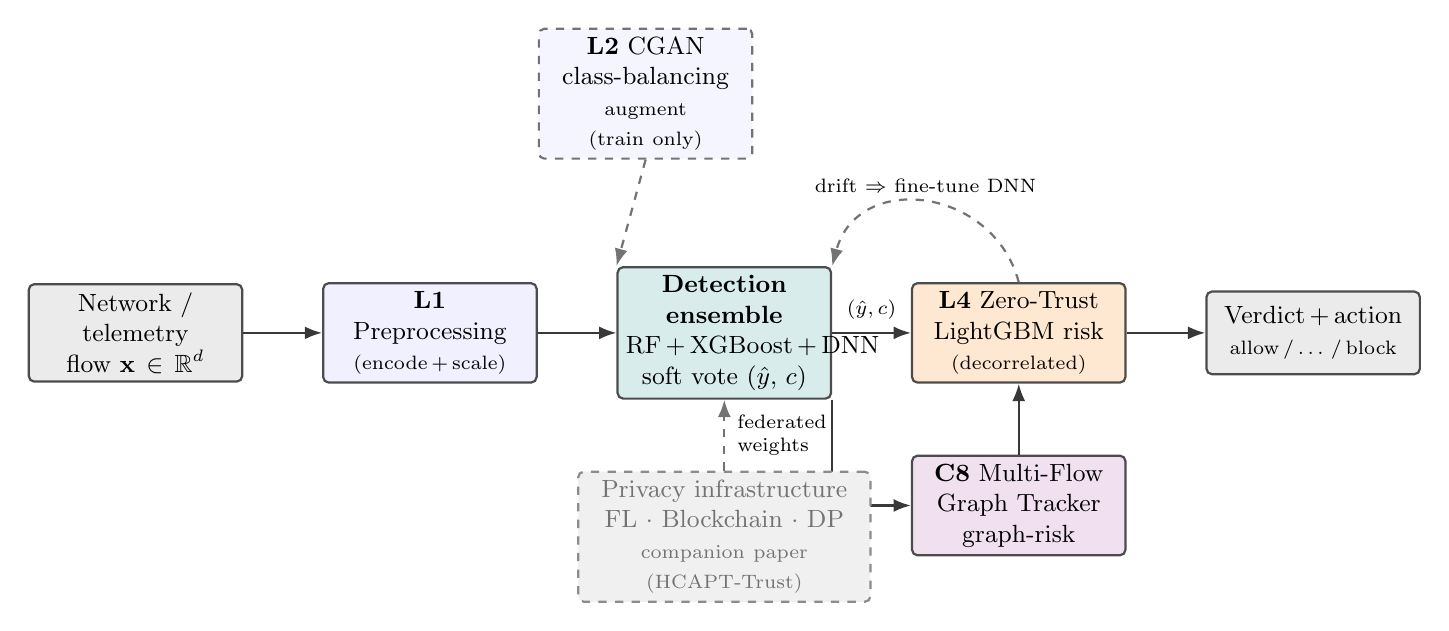
\begin{tikzpicture}[
  font=\small,
  >={Latex[length=2.2mm]},
  node distance=9mm and 10mm,
  block/.style={rectangle, rounded corners=2pt, draw=black!70, thick,
    fill=blue!6, minimum height=1.05cm, text width=2.5cm, align=center, inner sep=3pt},
  io/.style   ={block, fill=black!8},
  det/.style  ={block, fill=teal!15},
  zt/.style   ={block, fill=orange!18},
  train/.style={block, fill=blue!4, dashed, draw=black!55},
  side/.style ={block, fill=violet!12},
  comp/.style ={rectangle, rounded corners=2pt, draw=black!45, dashed, thick,
    fill=black!6, text=black!55, minimum height=1cm, text width=3.5cm, align=center, inner sep=3pt},
  arr/.style  ={->, thick, draw=black!78},
  feed/.style ={->, thick, dashed, draw=black!55},
]

% ---- main detection flow (left to right) ----
\node[io]  (in)  {Network / telemetry\\ flow $\mathbf{x}\in\mathbb{R}^{d}$};
\node[block, right=of in]  (l1)  {\textbf{L1}\\ Preprocessing\\ {\scriptsize (encode\,+\,scale)}};
\node[det,   right=of l1]  (ens) {\textbf{Detection ensemble}\\ RF\,+\,XGBoost\,+\,DNN\\ soft vote $(\hat y,\,c)$};
\node[zt,    right=of ens] (zt)  {\textbf{L4} Zero-Trust\\ LightGBM risk\\ {\scriptsize (decorrelated)}};
\node[io,    right=of zt]  (out) {Verdict\,+\,action\\ {\scriptsize allow\,/\,\ldots\,/\,block}};

\draw[arr] (in)  -- (l1);
\draw[arr] (l1)  -- (ens);
\draw[arr] (ens) -- node[above=1pt,font=\scriptsize]{$(\hat y,c)$} (zt);
\draw[arr] (zt)  -- (out);

% ---- CGAN augmentation (training-time only), above-left of the ensemble ----
\node[train, above=1.35cm of ens, xshift=-10mm] (gan)
      {\textbf{L2} CGAN\\ class-balancing\\ {\scriptsize augment (train only)}};
\draw[feed] (gan.south) -- (ens.north west);

% ---- self-learning drift loop: Zero-Trust -> ensemble (arcs clear on the right) ----
\draw[feed] (zt.north) to[out=105,in=75,looseness=1.35]
      node[pos=0.5,above,font=\scriptsize]{drift $\Rightarrow$ fine-tune DNN} (ens.north east);

% ---- Multi-Flow Graph Tracker (Component 8): parallel risk channel ----
\node[side, below=of zt] (gt) {\textbf{C8} Multi-Flow\\ Graph Tracker\\ graph-risk};
\draw[arr] (ens.south east) |- (gt.west);
\draw[arr] (gt.north) -- (zt.south);

% ---- companion privacy infrastructure (greyed): federated DNN weights ----
\node[comp, below=of ens] (priv) {Privacy infrastructure\\ FL $\cdot$ Blockchain $\cdot$ DP\\ {\scriptsize companion paper (HCAPT-Trust)}};
\draw[feed] (priv.north) -- node[right=1pt,font=\scriptsize,align=left]{federated\\ weights} (ens.south);

\end{tikzpicture}
\end{document}
